\chapter{Testing}

\section{Test plan}
\begin{longtable}{ | p{4cm} | p{4cm} | p{4cm} | }
	\hline
	\textbf{Test series} & \textbf{Purpose} & \textbf{Forms tested}\\
	\endfirsthead
	\hline
	\textbf{Test series (cont.)} & \textbf{Purpose (cont.)} & \textbf{Forms tested (cont.)}\\
	\endhead
	\hline
	1 &  Flow of control tests: menus, buttons, forms linking to each other and opening when required. & All of the forms.\\
	\hline
	2 & Input validation: textboxes and user input. & All of the data input forms.\\
	\hline
	3 & Tab order. & All of the data input forms.\\
	\hline
	4 & Search box testing. & frmList.\\
	\hline
	5 & Database data manipulation: fields inserted correctly, no crashing of the program. & Data input and retreival forms.\\
	\hline
	6 & Word document manipulation: test that they open and close perfectly and that all the required data is inserted in them. & frmReportQuote, frmReportLog, frmReportInvoice.\\
	\hline
\end{longtable}

\section{Test data}
\begin{longtable}{ | p{4cm} | p{4cm} | p{4cm} | p{4cm} | }
	\hline
	\textbf{Data number} & \textbf{Normal} & \textbf{Boundary} & \textbf{Erroneous}\\
	\endfirsthead
	\textbf{Data number (cont.)} & \textbf{Normal (cont.)} & \textbf{Boundary (cont.)} & \textbf{Erroneous (cont.)}\\
	\endhead
	\hline
	1 & 01234567890123 & N\slash A & [empty]\\
	\hline
	2 & Hello@example.com & N\slash A. & Helloexample.com\\
	\hline
	3 & Dung & N\slash A & [empty]\\ % Text customer name fields etc.
	\hline
	4 & 01473 847382 & N\slash A & [empty]\\
	\hline
	5 & 25 & $-1$ & q2\\
	\hline
\end{longtable}

\section{Test details}

The colour-coded key:
\begin{longtable}{ | p{4cm} | p{4cm} | p{4cm} | }
	\hline
	\textbf{\textcolor{red}{ERRONEOUS DATA}} & \textbf{\textcolor{blue}{BOUNDARY DATA}} & \textbf{\textcolor{magenta}{NORMAL DATA}}\\
	\hline
\end{longtable}

\textsl{Please turn over for further test details\ldots}
\begin{landscape}
\begin{longtable}{ | p{1cm} | p{2.5cm} | p{4cm} | p{1cm} | p{3cm} | p{3cm} | p{1.5cm} | p{1cm} |}
	\hline
	\textbf{Test number} & \textbf{Form} & \textbf{Purpose} & \textbf{Test data} & \textbf{Expected result} & \textbf{Actual result} & \textbf{Evidence} & \textbf{Pass\slash Fail}\\
	\endfirsthead
	\hline
	\textbf{Test number (cont.)} & \textbf{Form (cont.)} & \textbf{Purpose (cont.)} & \textbf{Test data (cont.)} & \textbf{Expected result (cont.)} & \textbf{Actual result (cont.)} & \textbf{Evidence (cont.)} & \textbf{Pass\slash Fail (cont.)}\\
	\endhead
	\hline
	1.1 & frmMainMenu & Test that every button clicked opens the expected form. & N\slash A & \textcolor{red}{N\slash A}; \textcolor{blue}{N\slash A}; \textcolor{magenta}{The Add button opens frmAdd, the Remove button opens frmRemove, the List button opens frmList, the Report Forms button opens frmReportMenu, and the Quit button closes the program.} & \textcolor{red}{N\slash A}; \textcolor{blue}{N\slash A}; \textcolor{magenta}{As expected.} & & Pass.\\
	\hline
	2.1 & frmAddCustomer & Make sure that MPAN number input isn't NULL, i.e. that the program does not error. & Test data 1. & \textcolor{red}{An error message displays if the input is NULL.}; \textcolor{blue}{N\slash A}; \textcolor{magenta}{The MPAN number field has data in it, so does not crash but inserts the data if all other checks are correct.} & \textcolor{red}{As expected.}; \textcolor{blue}{N\slash A}; \textcolor{magenta}{As expected.} &  & Pass.\\
	\hline
	2.2 & frmAddCustomer & Make sure that the email address contains an `@' symbol; if it does not, error. & Test data 2. & \textcolor{red}{An error message displays if the email address textbox is blank or does not contain an at symbol}; \textcolor{blue}{N\slash A}; \textcolor{magenta}{The email address contains an at symbol, so no errors display and the data is inserted into the database if all other checks are successful.} & \textcolor{red}{As expected.}; \textcolor{blue}{N\slash A}; \textcolor{magenta}{As expected.} & See screenshot~\ref{fig:test_2dot2} on page~\pageref{fig:test_2dot2}. & Pass.\\
	\hline
	2.3 & frmAddCustomer & Make sure that neither the name nor the billing address textboxes are left blank. & Test data 3. & \textcolor{red}{An error message displays if the textboxes are blank.}; \textcolor{blue}{N\slash A}; \textcolor{magenta}{None of the textboxes are blank, so no errors display and the data is inserted into the database if all other checks are successful.} & \textcolor{red}{As expected.}; \textcolor{blue}{N\slash A}; \textcolor{magenta}{As expected.} &  & Pass.\\
	\hline
	2.4 & frmAddCustomer & Make sure that the telephone number boxes are not left blank. & N\slash A & \textcolor{red}{An error message displays if the telephone number texboxes are blank.}; \textcolor{blue}{N\slash A}; \textcolor{magenta}{None of the telephone number textboxes are blank, so no errors display and the data is inserted into the database if all other checks are successful.} & \textcolor{red}{As expected.}; \textcolor{blue}{N\slash A}; \textcolor{magenta}{As expected.} & & Pass.\\
	\hline
	2.5 & frmAddSupplier & Make sure that the telephone number boxes are not left blank. & N\slash A & \textcolor{red}{An error message displays if the telephone number texboxes are blank.}; \textcolor{blue}{N\slash A}; \textcolor{magenta}{None of the telephone number textboxes are blank, so no errors display and the data is inserted into the database if all other checks are successful.} & \textcolor{red}{As expected.}; \textcolor{blue}{N\slash A}; \textcolor{magenta}{As expected.} & & Pass.\\
	\hline
	2.6 & frmAddSupplier & Make sure that neither the name nor the supplier address, nor the contact name textboxes are left blank. & Test data 3. & \textcolor{red}{An error message displays if the textboxes are blank.}; \textcolor{blue}{N\slash A}; \textcolor{magenta}{None of the textboxes are blank, so no errors display and the data is inserted into the database if all other checks are successful.} & \textcolor{red}{As expected.}; \textcolor{blue}{N\slash A}; \textcolor{magenta}{As expected.} &  & Pass.\\
	\hline
	2.7 & frmAddComponent & Make sure that neither the name nor the component type textboxes are left blank. & Test data 3. & \textcolor{red}{An error message displays if the textboxes are blank.}; \textcolor{blue}{N\slash A}; \textcolor{magenta}{None of the textboxes are blank, so no errors display and the data is inserted into the database if all other checks are successful.} & \textcolor{red}{As expected.}; \textcolor{blue}{N\slash A}; \textcolor{magenta}{As expected.} &  & Pass.\\
	\hline
	2.8 & frmAddComponent & Make sure that only a positive numerical value is accepted in the kWp textbox. & Test data 5. & \textcolor{red}{An error message displays if the textbox does not contain a number.}; \textcolor{blue}{Error if the number entered by the user is negative.}; \textcolor{magenta}{None of the textboxes are blank and the kWp number is positive, so no errors display and the data is inserted into the database if all other checks are successful.} & \textcolor{red}{As expected.}; \textcolor{blue}{N\slash A}; \textcolor{magenta}{As expected.} & See the screenshot~\ref{fig:test_2dot8} on page~\pageref{fig:test_2dot8}. & Pass.\\
	\hline
	3.1 & frmAddCustomer & Test the tab order of the customer addition form: the tab order should be logical and tabs should go from one textbox to the one straight underneath it, and from the last textbox to the Save button and then to the Cancel button. & & This is simply a pass or fail test. & & & Pass.\\
	\hline
	3.2 & frmAddSupplier & Test the tab order of the supplier addition form: the tab order should be logical and tabs should go from one textbox to the one straight underneath it, and from the last textbox to the Save button and then to the Cancel button. & & This is simply a pass or fail test. & & & Pass.\\
	\hline
	3.3 & frmAddComponent & Test the tab order of the component addition form: the tab order should be logical and tabs should go from one textbox to the one straight underneath it, and from the last textbox to the Save button and then to the Cancel button. & & This is simply a pass or fail test. & & & Pass.\\
	\hline
	4.1 & frmList & Test the search box functionality. & Test data is in the database, from the frmAddCustomer tests: testing `banana'. & \textcolor{red}{The search functionality does not search for anything.}; \textcolor{blue}{The user entered `Ba' and not `Banana', so all of the results matching `Ba' even inside the strings were returned.}; \textcolor{magenta}{The searched string displays all of its variants for the user to select.} & \textcolor{red}{As expected.}; \textcolor{blue}{As expected.}; \textcolor{magenta}{As expected.} & See the screenshot~\ref{fig:test_4dot1} on page~\pageref{fig:test_4dot1}. & Pass.\\
	\hline
	5.1 & frmAddCustomer & Test that everything is inserted correctly into the database. & Test data used in test series 2. & \textcolor{red}{Erroneous data is input into the database---unexpected blank boxes due to validation failures, for example.}; \textcolor{blue}{N\slash A.}; \textcolor{magenta}{Everything is correctly inserted into the database.} & \textcolor{red}{As expected.}; \textcolor{blue}{As expected.}; \textcolor{magenta}{As expected.} & See screenshot~\ref{fig:test_5dot1} on page~\pageref{fig:test_5dot1}. & Pass.\\
	\hline
	6.1 & frmReportQuote, frmReportLog, frmReportInvoice & Test that the Word documents open and display at the click of the relevant buttons, and that they can be edited and printed. & Previously inserted data, from the database. & \textcolor{red}{The Word documents do not open; the program crashes.}; \textcolor{blue}{N\slash A.}; \textcolor{magenta}{The Word documents open and can be printed and edited and saved again.} & \textcolor{red}{As expected.}; \textcolor{blue}{N\slash A.}; \textcolor{magenta}{As expected.} & See screenshots~\ref{fig:test_6dot1} on page~\ref{fig:test_6dot1}. & Pass.\\
	\hline
\end{longtable}
\end{landscape}

(For the sake of brevity, I have only included evidence of a few tests of every form.)
\section{Associated screenshots}

\begin{figure}[ht]
	\centering
	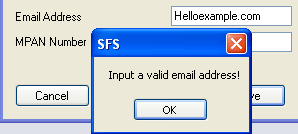
\includegraphics[scale=0.5]{test_2dot2}
	\caption{Email address error message.}
	\label{fig:test_2dot2}
\end{figure}

\begin{figure}[ht]
	\centering
	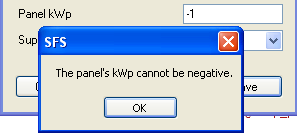
\includegraphics[scale=0.5]{test_2dot8}
	\caption{Boundary kWp data entry error.}
	\label{fig:test_2dot8}
\end{figure}

\begin{figure}[ht]
	\centering
	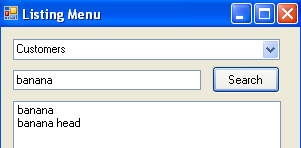
\includegraphics[scale=0.5]{test_4dot1}
	\caption{The search function succeeding.}
	\label{fig:test_4dot1}
\end{figure}

\begin{figure}[ht]
	\centering
	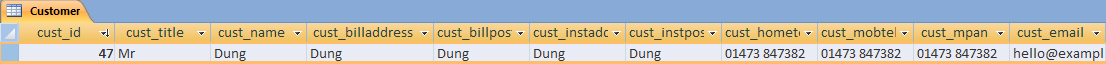
\includegraphics[scale=0.4]{test_5dot1}
	\caption{The customer data inserted correctly into the database.}
	\label{fig:test_5dot1}
\end{figure}

\begin{figure}[ht]
	\centering
	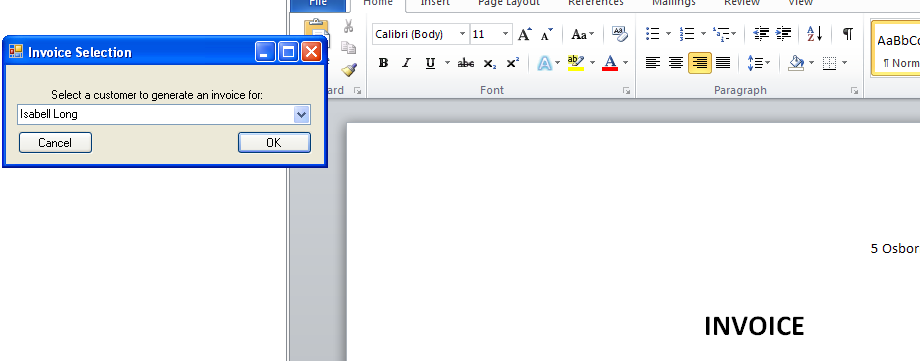
\includegraphics[scale=0.5]{invoice-IL-select-word_scrot}
	\caption{The invoice opening.}
	\label{fig:test_6dot1}
\end{figure}